\documentclass[12pt, a4paper]{book}
\usepackage[utf8]{inputenc}
\usepackage[T1]{fontenc}
\usepackage[default, oldstyle, scale=.95]{opensans} % police Open Sans
\usepackage{setspace}
\usepackage{amsmath}
\usepackage{amsfonts}
\usepackage{fancyhdr}
\usepackage{amssymb}
\usepackage[nottoc, notlof, notlot]{tocbibind}
\usepackage{xcolor} % où color selon l'installation
\definecolor{Prune}{RGB}{99,0,60} % l14-33 : couleurs de la charte graphique upsaclay
\definecolor{B1}{RGB}{49,62,72} 
\definecolor{C1}{RGB}{124,135,143}
\definecolor{D1}{RGB}{213,218,223}
\definecolor{A2}{RGB}{198,11,70}
\definecolor{B2}{RGB}{237,20,91}
\definecolor{C2}{RGB}{238,52,35}
\definecolor{D2}{RGB}{243,115,32}
\definecolor{A3}{RGB}{124,42,144}
\definecolor{B3}{RGB}{125,106,175}
\definecolor{C3}{RGB}{198,103,29}
\definecolor{D3}{RGB}{254,188,24}
\definecolor{A4}{RGB}{0,78,125}
\definecolor{B4}{RGB}{14,135,201}
\definecolor{C4}{RGB}{0,148,181}
\definecolor{D4}{RGB}{70,195,210}
\definecolor{A5}{RGB}{0,128,122}
\definecolor{B5}{RGB}{64,183,105}
\definecolor{C5}{RGB}{140,198,62}
\definecolor{D5}{RGB}{213,223,61}
\usepackage{mdframed}
\usepackage{multirow} %% Pour mettre un texte sur plusieurs rangées
\usepackage{multicol} %% Pour mettre un texte sur plusieurs colonnes
\usepackage{scrextend} %Forcer la 4ème  de couverture en page pair
\usepackage{tikz}
\usepackage{graphicx}
\usepackage[absolute]{textpos} 
\usepackage{colortbl}
\usepackage{array}
\usepackage{geometry}
\usepackage{titlesec}
\usepackage{caption}
\captionsetup[figure]{font={stretch=1.5}}
\usepackage{hyperref}
\hypersetup{ % paramétrage couleur des liens hypertextes, toujours garder colorlinks=true
    colorlinks=true,
    linkcolor=black,
    urlcolor=purple,
    citecolor=purple
}

\pagestyle{plain} % pour ne garder que les n°de page en milieu-bas et supprimer les indications de chapitre en marge haute

\begin{document}

\begin{titlepage}

%\thispagestyle{empty}

\newgeometry{left=6cm,bottom=2cm, top=1cm, right=1cm}

\tikz[remember picture,overlay] \node[opacity=1,inner sep=0pt] at (-13mm,-135mm){
\includegraphics{images/Frame-ups.pdf}};

%*****************************************************
%******** NUMÉRO D'ORDRE DE LA THÈSE À COMPLÉTER *****
%******** POUR LE SECOND DÉPOT                   *****
%*****************************************************

\color{white}

\begin{picture}(0,0)
\put(-152,-743){\rotatebox{90}{\Large \textsc{THESE DE DOCTORAT}}} \\
\put(-120,-743){\rotatebox{90}{NNT : 2020UPASA001}}
\end{picture}


%*****************************************************
%******************** TITRE **************************
%*****************************************************

\flushright
\vspace{10mm} % à régler éventuellement
\color{Prune}
\fontfamily{cmss}\fontseries{m}\fontsize{22}{26}\selectfont
  \Huge Geographic and socio-demographic disparities in oncology care pathways \\

\normalsize
\color{black}
\Large{\textit{
Etude des disparités géographiques et socio-démographiques dans les parcours de soins en oncologie}} \\
%*****************************************************

\fontfamily{fvs}\fontseries{m}\fontsize{8}{12}\selectfont

\vspace{1.5cm}

\normalsize
\textbf{Thèse de doctorat de l'université Paris-Saclay} \\

\vspace{6mm}

\small École doctorale n$^{\circ}$ d'accréditation, dénomination et sigle\\
\small Spécialité de doctorat: voir annexe\\
\small Graduate School : voir annexe, Référent : voir annexe \\
\vspace{6mm}

\footnotesize Thèse préparée dans la (ou les) unité(s) de recherche Nom(s) (voir annexe), sous la direction de Prénom NOM, titre du directeur ou de la directrice de thèse, la co-direction de Prénom NOM, titre du co-directeur ou de la co-directrice de thèse, le co-encadrement de Prénom NOM, titre, du co-encadrant ou de la co-encadrante ou la co-supervision de Prénom NOM, titre, du tuteur ou de la tutrice (en cas de partenariat industriel) \\
\vspace{15mm}

\textbf{Thèse soutenue à Paris-Saclay, le JJ mois AAAA, par}\\
\bigskip
\Large {\color{Prune} \textbf{Eric DAOUD-ATTOYAN}} %

%************************************
\vspace{\fill} % ALIGNER LE TABLEAU EN BAS DE PAGE
%************************************

\bigskip

\flushleft
\small \textbf{Composition du jury}\\
\vspace{2mm}
\scriptsize
\begin{tabular}{|p{7cm}l}
\arrayrulecolor{Prune}
\textbf{Prénom Nom} &   Président ou Présidente\\ 
Titre, Affiliation & \\
\textbf{Prénom Nom} &  Rapporteur \& Examinateur / trice \\ 
Titre, Affiliation   &   \\ 
\textbf{Prénom Nom} &  Rapporteur \& Examinateur / trice \\ 
Titre, Affiliation  &   \\ 
\textbf{Prénom Nom} &  Examinateur ou Examinatrice \\ 
Titre, Affiliation   &   \\ 
\textbf{Prénom Nom} &  Examinateur ou Examinatrice \\ 
Titre, Affiliation   &   \\ 
\textbf{Prénom Nom} &  Directeur ou Directrice de thèse \\ 
Titre, Affiliation   &   \\ 

\end{tabular} 

\end{titlepage}

%********************
%***** Chapters *****
%********************

\newgeometry{top=4cm, bottom=4cm, left=2cm, right=2cm}

\begin{singlespace}
\setstretch{1.5}

\chapter{Introduction}

There will be an estimated 382,000 new cases of incident cancer and 157,400
deaths in 2018 in France. The French Cancer Plan \cite{buzyn_plan_2014}
2014-2019 announces the objectives to be implemented in the fight against cancer
in France. In particular, objectives 2 and 7 insist on the quality of the care
pathway: they aim respectively to ``guarantee the quality and safety of care''
and ``ensure comprehensive and personalized care''.

\section{Care pathways}

In order to standardize the care pathway while personalizing management, care
trajectories have been established. The definition of these optimal care
trajectories is based on national and international good practice
recommendations.

\section{Disparities in care pathways}

\ac{inca} has published several studies comparing care pathways in France with
national and international recommendations. One of them concerns the time
required for the management of breast and lung cancer. This study found
differences according to the status of the institution of first therapeutic
management or the region \cite{bernard_ledesert_etude_2012}. However, the study
does not explain these differences, in particular because of the lack of
availability of socio-demographic indicators. Today, there are several public
data sources that provide access to these indicators at the municipality level.
Incorporating additional data sources could lead to better understanding of
where these disparities in management come from according to the care
facilities. Indeed, the multiplicity of care centers, their types, the distance
of the care centers from the patients' homes and the location of treatments are
all factors that can degrade the care pathway and impact the prognosis of cancer
patients.

\subsection*{Geographical disparities}

A study analyzed the care pathways in Tanzania for patients with tuberculosis
\cite{mhalu_pathways_2019}. The study highlights the complexity of the pathways
from the first symptoms to diagnosis and the high cost of accessing health care
facilities.

Several studies have investigated the optimal distribution of care centers in
different countries, as well as their accessibility by road or public transport.
A study of health care facilities for the city of Shenzhen in China showed
differences in access to health care depending on the mode of transport used. It
appears that public transport users are at a disadvantage compared to patients
with a car \cite{tao_spatial_2018}. Mandel et al \cite{mandel_optimizing_2018}
showed that an application similar to Google Maps for guiding patients to
different care centers in a multi-site hospital reduces patient travel time. In
particular, the application uses real-time traffic data for referral. Jia et al
\cite{jia_selecting_2014} proposed a method to select the optimal care center
using several criteria such as geographic accessibility and service quality. In
particular, transportation networks such as high-speed lines and highways are
taken into account in the center selection.

\subsection*{Socio-demographic disparities}

Various studies have investigated the impact of socio-demographic factors on the
course of care and survival prognosis of patients. An American study on lung
cancer patients showed that good physical and intellectual conditions were
linked to better survival from the disease
\cite{pierzynski_socio-demographic_2018}.

A second study shows differences in access to care related to ethnicity for
patients with psychosis \cite{anderson_meta-analysis_2014}.

Even though the burden of cancer is easing in the United States, the decline is
unequal among different racial, ethnic and socio-economic groups
\cite{viswanath_science_2005}.

The aim of this study was to examine the impact of patient demographics, tumor
characteristics, and treatment type on time to treatment (TTT) in patients with
breast cancer treated at a safety net medical center with a diverse patient
population. Longer median TTT was noted for Black and single patients
\cite{khanna_impact_2017}.

\subsection*{Gender-related disparities}

Gender appears to have an impact on care pathways. For example, men may have
difficulty talking about their symptoms, fearing that it will be perceived as a
sign of weakness; whereas women who require care are more likely to be neglected
\cite{ferrari_gender_2018}. Indeed, women with myocardial infarction have a
higher mortality rate than men, and this discrepancy appears to be partially due
to delayed diagnosis and access to appropriate care
\cite{bugiardini_delayed_2017}. Similarly, a pediatric study of kidney
transplantation showed that young girls had less rapid access to transplantation
than young boys. This is partly due to non-medical reasons such as parental and
practitioner behavior regarding organ donation \cite{hogan_j_gender_2016}. More
specifically, the gender of the patient could have an impact on the oncology
care pathway. Indeed, several studies show that women's treatment for several
types of cancers is suboptimal. This would at least partially explain why their
chances of survival from these diseases are lower than those of men
\cite{park_a_undertreatment_2019,carter_paulson_e_gender_2009,rose_sex_2016}.
The above examples suggest that patient survival could be improved by taking
gender into consideration in the care pathway. However, at present, gender
differences in the oncology care pathway are barely explored.

\chapter{Accessibility to oncology care}

\section{Context}

\subsection{Motivation}

While a lot of the ongoing research is focusing on finding new cancer treatments, accessibility to oncology care receives less attention. Yet, several studies have showed that access to health services plays a key role in cancer survival. For instance, geographic residency status and social environment seem to explain treatment and prognosis disparities for patients with non-small cell lung cancer \cite{johnson_treatment_2014}. In France, increases in travel times to health services were associated with lower survival rates for patients with a colorectal cancer \cite{dejardin_influence_2014}. In New Zealand, living in deprived areas, far from a cancer center or from primary care was associated with lower survival chances for patients with colorectal, lung and prostate cancers \cite{haynes_cancer_2008}. 

\subsection{Accessibility definition}

Accessibility refers to the relative ease by which services can be reached from a given location \cite{wang_measurement_2012}. Accessibility can be defined by spatial factors, determined by where you are; and non-spatial factors, determined by who you are \cite{khan_integrated_1992}. Spatial accessibility methods assess the availability of supply locations from demand locations, connected by a travel impedance metric. Supply locations are characterized by their capacity or quantity of available resource. Similarly, demand locations are characterized by their population. Such methods have been successfully used to measure access to healthcare, such as primary care \cite{guagliardo_spatial_2004} or oncology care \cite{wang_measurement_2012,zahnd_spatial_2021,alahmadi_spatial_2013} in several countries including France \cite{launay_methodology_2019,gusmano_disparities_2014,gao_assessment_2016}. In what follows, we restrict accessibility to spatial accessibility and use both terms interchangeably.

\subsection{Spatial accessibility methods}

There are several ways to compute accessibility to healthcare \cite{guagliardo_spatial_2004}. The easiest and most straightforward methods are computed within bordered areas, like provider-to-population ratios in each municipality. While they are very intuitive, these methods do not account for border crossing, or travel impedance, which makes them less accurate. Recently, a new type of method has been developed and is now used in most spatial accessibility papers. This algorithm is called Two Step Floating Catchment Area (2SFCA) \cite{luo_using_2004}. It is a two-step method that first computes a provider-to-population ratio for each provider location. In the second step, for each population location, an accessibility score is obtained by summing the provider-to-population ratios. For the algorithm to work, a catchment threshold (distance or travel time) must be set. Above this threshold, a provider location is considered unreachable from the population location, and vice versa. The 2SFCA method does not account for distance decay: a care center is either reachable or not. The Enhanced Two Step Floating Catchment Area (e2SFCA) \cite{luo_enhanced_2009} addresses this limitation by applying weights to differentiate travel zones in both steps. 
We now explain more formally how to compute eS2FCA scores. Consider $P_i$ the population at location $i$, with $1 \leq i \leq n$ where n is the number of population locations. Similarly, consider $S_u$ the capacity of care center $u$, with $1 \leq u \leq m$ where $m$ is the number of care centers. Finally, let $d_{iu}$ be the matrix of size $n \times m$ containing the distances between location i and care center u. We consider r sub-catchment zones each associated with a weight $W_s$, and a distance $D_s$, with $1 \leq s \leq r$, such that $D_1 D_2 < ... < D_r$ and $W_1 > W_2 > ... > W_r$. The resulting r travel intervals are $I_1=[0, D_1], I_2=[D_1, D_2 ],… ,I_r=[D_{r-1}-,D_r]$. The accessibility $A_i$ of a population location $i$ is computed in two steps:

\begin{itemize}
    \item Step 1: for every care center u, compute its weighted capacity-to-population ratio $R_u$. 
    
    \begin{equation}
    R_u =  \frac{S_u}{\sum_{s=1}^{r} W_s \sum_{i, d_{iu} \in I_s} P_i}
    \end{equation}
    
    \item Step 2: for every population location, compute $A_i$ as the sum all the weighted $R_u$ of the reachable care centers. 
    
    \begin{equation}
    A_i = \sum_{s=1}^{r} W_s \sum_{u, d_{iu} \in I_s} R_u
    \end{equation}
\end{itemize}

\section{Spatial accessibility to oncology care centers in metropolitan France}
\chapter{Accessibility optimization}

\section{Context}

\subsection{Motivation}

Uneven distributions of population and health-care providers lead to geographic disparity in accessibility for patients \cite{wang_why_2020}. For instance, Weiss et al. \cite{weiss_global_2020} showed that 8.9\% of the global population could not reach healthcare within one hour if they have access to motorized transport. In Germany, Bauer et al. \cite{bauer_spatial_2020} shown that 10\% of the population lived in areas with low accessibility for internal medicine and surgery. Location-allocation algorithms \cite{church_location_1999} can optimize the distribution and supply of health providers to reduce accessibility disparities. These algorithms seek the optimal placement of facilities for a desirable objective under certain constraints \cite{wang_measurement_2012}. For instance, Luo et al. developed an optimization algorithm to improve the healthcare planning in rural China by finding the best place and capacity for new health facilities \cite{luo_integrating_2014}. Tao et al. worked on a spatial optimization model to maximize equity in accessibility to residential care facility in Beijing, China \cite{tao_spatial_2014}. When optimizing health accessibility, there are two competing goals: equity and efficiency \cite{krugman_opinion_2013,meyer_equity_2008}. Equity may be defined as equal access to healthcare for everyone \cite{culyer_equity_1993}. An efficient situation is when everything has been done to help any person without harming anyone else \cite{hemenway_optimal_1982}. While some argue that efficiency should be ad-dressed in priority \cite{hemenway_optimal_1982}, others agree that equity is a matter of ethical obligation, especially in public health \cite{fried_rights_1975, oliver_equity_2004}.

\subsection{Location-allocation algorithms}

Regarding efficiency optimization, the most popular algorithms are p-median, location set covering problem (LSCP) and maximum covering location problem (MCLP). The p-median algorithm minimizes the weighted sum of distances between users and facilities \cite{murad_using_2021}. LSCP minimizes the number of facilities needed to cover all demand \cite{shavandi_fuzzy_2006}. MCLP maximizes the de-mand covered within a desired distance or time threshold by locating a given number of facilities \cite{casado_heuristical_2005}. 
To reach equal access to healthcare, quadratic programming has been used to  minimize the variance of accessibility scores defined by the 2SFCA \cite{wang_planning_2013}. Similarly, a Particle Swarm Optimization (PSO) algorithm was developed to minimize the total square difference between the accessibility score of each demand location and the weighted average accessibility score \cite{tao_spatial_2014}. Finally, a two-step optimization algorithm has been developed to address the dual objectives of efficiency and equality, by first choosing where to site new hospitals and then deciding which capacity they should have \cite{luo_two-step_2017,li_two-step_2017}.

\section{Care centers characterization}

There are many care centers in France, which do not share the same degree of oncology specialization. Therefore, we first run a clustering algorithm to automatically group the care centers based on their medical statistics and attributes. Using these clusters, we label the care centers in terms of hospital development and oncology specialization. 

\begin{figure}[t]
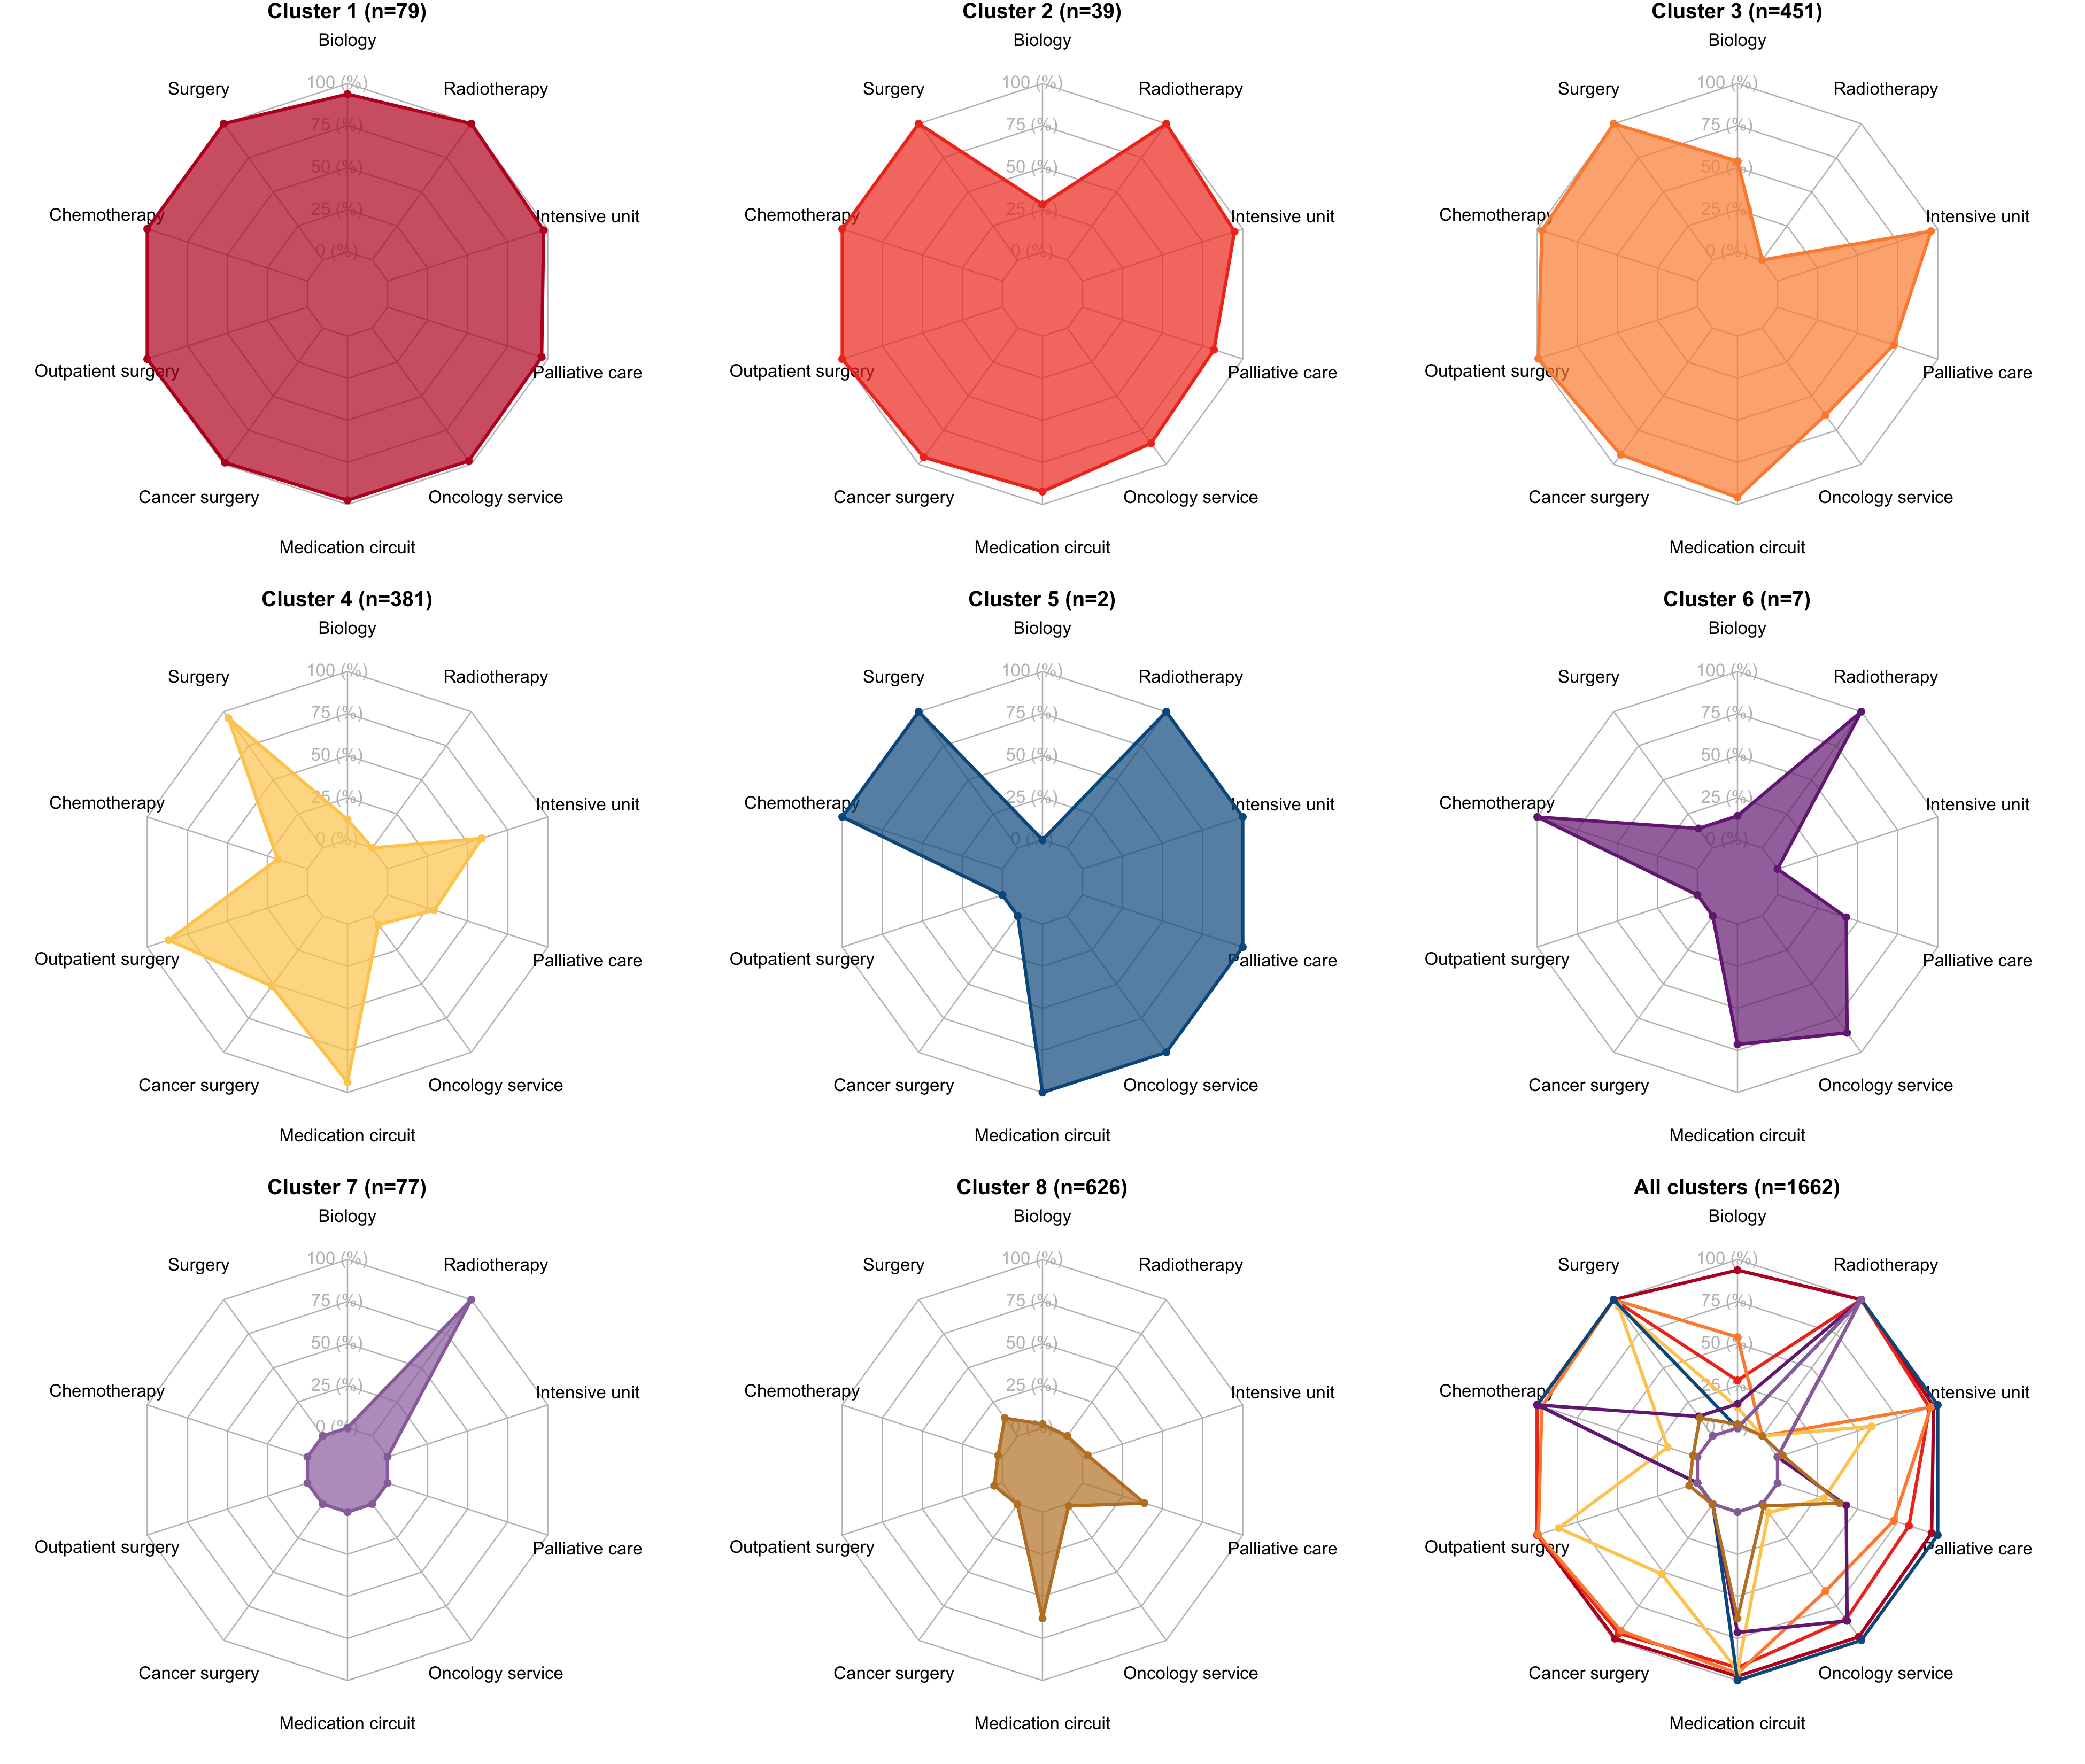
\includegraphics[width=\textwidth]{images/camion/fig1_clusters_services.png}
\centering
\caption{
Distribution of the care centers services and equipment per cluster. Each radar plot axis shows the percentage of the care centers within the cluster that have the corresponding attribute. In Cluster 1, the care centers have all the listed services. In cluster 8, the centers have almost none of the services. Care centers from cluster 1 (n=79) and cluster 2 (n=39) are the most suit-ed for oncology care.
}
\end{figure}
\chapter{Optimizing patients travel}

\end{singlespace}

%%%%%%%%%%%%%%%%%%%%%%%%%%%%%%%%%%%%%%%%%%%%%%%%%%%%%%%%%%%%%%%
% 4eme de couverture
\Ifthispageodd{\newpage\thispagestyle{empty}\null\newpage}{}
\thispagestyle{empty}
\newgeometry{top=1.5cm, bottom=1.25cm, left=2cm, right=2cm}
\fontfamily{rm}\selectfont

\lhead{}
\rhead{}
\rfoot{}
\cfoot{}
\lfoot{}

\noindent 
%************************
%***** LOGO DE L'ED *****
%************************

\includegraphics[height=2.45cm]{images/logos/logo_usp_CBMS.png}
\vspace{1cm}
%*****************************************************
\fontfamily{cmss}\fontseries{m}\selectfont

\small

%*********************
%***** ABSTRACTS *****
%*********************

\begin{mdframed}[linecolor=Prune,linewidth=1]

    \textbf{Titre:} Etude des disparités géographiques et socio-démographiques dans les parcours de soins en oncologie.

    \noindent \textbf{Mots clés:} 3 à 6 mots clefs (version en français)

    \vspace{-.5cm}
    \begin{multicols}{2}
        \noindent \textbf{Résumé:} On estime à 382 000 le nombre de nouveaux cas de
        cancers incidents et à 157 400 le nombre de décès en 2018 en France. Le Plan
        Cancer 2014-2019 annonce les objectifs à mettre en oeuvre dans la lutte contre le
        cancer en France. En particulier, les objectifs 2 et 7 insistent sur la qualité
        du parcours de soin : ils ambitionnent respectivement de ``garantir la qualité
        et la sécurité des prises en charge'' et ``assurer des prises en charge globales
        et personnalisés''. Dans le but de standardiser le parcours de soin tout en
        personnalisant la prise en charge, des trajectoires de soin ont été instaurées.
        La définition de ces trajectoires de soin optimales s'appuie sur des
        recommandations de bonnes pratiques nationales et internationales. Nous
        proposons d'étudier en détails les disparités géographiques et
        socio-démographiques dans les parcours de soin des patients atteints d'un cancer
        en France. Dans un premier temps, nous chercherons à caractériser les
        établissements de santé en France à partir de leur activité en oncologie. Puis,
        nous étudierons la distribution de ces centres sur le territoire, afin de mettre
        en évidence d'éventuelles disparités dans l'accès à ceux-ci. Enfin, nous
        tenterons de proposer un algorithme de recommandations de centres de soins, à
        partir des données du Système National des Données de Santé (SNDS). Cet
        algorithme aura pour but de guider les patients vers le centre optimal, en vue
        de maximiser la qualité du parcours de soins.

    \end{multicols}

\end{mdframed}


\vspace{8mm}

\begin{mdframed}[linecolor=Prune,linewidth=1]

\textbf{Title:} Geographic and socio-demographic disparities in oncology care pathways.

\noindent \textbf{Keywords:} 3 à 6 mots clefs (version en anglais)

\vspace{-.5cm}
\begin{multicols}{2}
\noindent \textbf{Abstract:} In France, during year 2018, there was 382,000 new cancer cases and 157,400 deaths. The 2014-2019 Cancer Plan sets new objectives for cancer care in France. In particular, objectives 2 and 7 emphasize the quality of the care pathways: they aim respectively to guarantee the quality and safety of care and ensure comprehensive and personalized care. In order to standardize the care pathways while personalizing care, care trajectories have been introduced. The definition of these optimal care trajectories is based on national and international good practice recommendations. We propose to study in detail the geographical and socio-demographic disparities in the care pathways of cancer patients in France. First, we will try to characterize the health care institutions in France based on their oncology activity. Then, we will study the distribution of these centers on the territory, in order to highlight possible disparities in access to them. Finally, we will try to propose a care center recommendation algorithm, using the French social security database (SNDS). This algorithm will aim at guiding patients towards the optimal center, in order to maximize the quality of the care pathways.

\end{multicols}
\end{mdframed}

\titleformat{\chapter}[hang]{\bfseries\Large\color{Prune}}{\thechapter\ -}{.1ex}
{\vspace{0.1ex}
}
[\vspace{1ex}]
\titlespacing{\chapter}{0pc}{0ex}{0.5pc}

\titleformat{\section}[hang]{\bfseries\normalsize}{\thesection\ .}{0.5pt}
{\vspace{0.1ex}
}
[\vspace{0.1ex}]
\titlespacing{\section}{1.5pc}{4ex plus .1ex minus .2ex}{.8pc}

\titleformat{\subsection}[hang]{\bfseries\small}{\thesubsection\ .}{1pt}
{\vspace{0.1ex}
}
[\vspace{0.1ex}]
\titlespacing{\subsection}{3pc}{2ex plus .1ex minus .2ex}{.1pc}

%**********************
%***** References *****
%**********************

\newgeometry{top=4cm, bottom=4cm, left=2cm, right=2cm}
\bibliographystyle{vancouver}
\bibliography{references.bib}

%***************
%***** TOC *****
%***************

\newgeometry{top=4cm, bottom=4cm, left=2cm, right=2cm}
\tableofcontents

\end{document}